\documentclass{article}
\usepackage[utf8]{inputenc}
\usepackage[T1]{fontenc}
%\usepackage[ngerman]{babel}
\usepackage{graphicx}
\usepackage{geometry}
\usepackage{pgfplots}
\pgfplotsset{compat=1.18}
\geometry{margin=25mm}

\newcommand{\AuthorName}{Leonard Röpcke\\Klasse TG-J2b}
\newcommand{\Institute}{Zepellin Gewerbeschule Konstanz}
\newcommand{\Subtitle}{Die Wissenschaft der Zahlen}
\newcommand{\MyDate}{\today}

\begin{document}
\begin{titlepage}
  \centering
  {\scshape\LARGE \Institute \par}
  \vspace{2.5cm}
  {\huge\bfseries Mathematik\par}
  \vspace{0.8cm}
  {\Large\itshape \Subtitle \par}
  \vfill
  {\Large Autor\par}
  {\Large \AuthorName \par}
  \vspace{1cm}
  {\Large Datum\par}
  {\Large \MyDate \par}
  \vfill
  % Optional: Bild einfügen (Datei hinzufügen oder Zeile auskommentieren)
  % \includegraphics[width=6cm]{example-image}
  \vspace{1cm}
  {\small }
  %unten am anfang
\end{titlepage}
\tableofcontents
\newpage

\section{Stochastik}
\subsection{Biominalverteilung}
\subsubsection{Beispiel: Uhr tragen}
In einer Schule werden \( n = 1000 \) Schülerinnen und Schüler gefragt, ob sie eine Uhr tragen.  
Die Wahrscheinlichkeit hierfür beträgt \( p = 0{,}45 \).
Gesucht ist die Wahrscheinlichkeit, dass die Anzahl der Uhrenträger:innen maximal um \( 3\sigma \) abweicht.

\[
\mu = n \cdot p = 1000 \cdot 0{,}45 = 450
\]
\[
\sigma = \sqrt{n \cdot p \cdot (1 - p)} = \sqrt{1000 \cdot 0{,}45 \cdot 0{,}55} \approx 15{,}73
\]
\[
3\sigma \approx 3 \cdot 15{,}73 = 47{,}19
\]

\noindent
\textbf{Mit der kumulierten Binomialverteilung:}\\
Mit dem Taschenrechner (gerundetes \(\sigma\) auf zwei Nachkommastellen) ergibt sich eine Wahrscheinlichkeit von etwa
\[
P(|X - \mu| \leq 3\sigma) \approx 0{,}9973 \quad \text{bzw. } 99{,}73\%.
\]

\medskip
\noindent
\textbf{Mit der kumulierten Normalverteilung:}
\[
P(402 \leq X \leq 497)
= \int_{402{,}5}^{497{,}5} \varphi(x) \, dx
\approx 0{,}9987 - 0{,}0012 = 0{,}9975 \quad \text{bzw. } 99{,}75\%.
\]
\noindent
Damit beträgt die Wahrscheinlichkeit, dass die Anzahl der Uhrenträger:innen maximal um \( 3\sigma \) abweicht, etwa \( 99{,}75\% \).
Hinweis: Es wird eine sogennate Stetigkeitskorrektur durchgeführt, indem 0,5 zu den Grenzen addiert bzw. subtrahiert wird.

\textbf{mit der Sigma-Regel:}
\[
p(|X - \mu| \leq 3\sigma) \approx 0{,}9973 \quad \text{bzw. } 99{,}73\%.
\]

\subsection{Wahrscheinlichkeiten bei kontinuierlichen Größen}
Die Normalverteilung hat den Vorteil, dass sie insbessondere bei nicht-diskreten, also kontinuierlichen
Größen verwendet werden kann. Beispiele hierfür sind:

\subsubsection{Körpergwecht von erwachsenen Männern}
Voraussetzungen:
\begin{itemize}
    \item Das Körpergewicht muss normalverteilt sein.
\end{itemize}

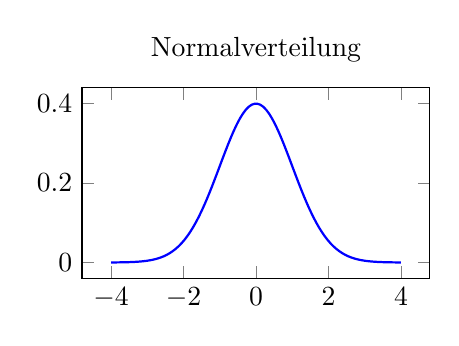
\begin{tikzpicture}
    \begin{axis}[
        width=6cm,
        height=4cm,
        domain=-4:4,
        samples=100,
        %xlabel=$x$,
        %ylabel={$f(x)$},
        title={Normalverteilung},
    ]
        \addplot[blue, thick] {1/sqrt(2*pi)*exp(-x^2/2)};
    \end{axis}
\end{tikzpicture}
\hspace{1cm}
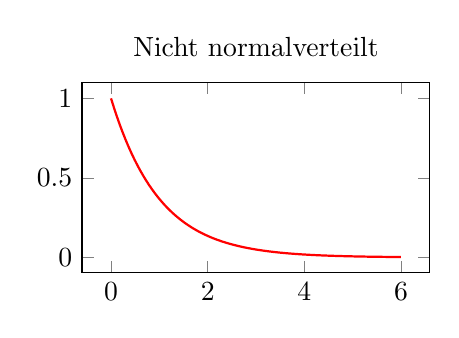
\begin{tikzpicture}
    \begin{axis}[
        width=6cm,
        height=4cm,
        domain=0:6,
        samples=100,
        %xlabel=$x$,
        %ylabel={$f(x)$},
        title={Nicht normalverteilt},
    ]
        % Beispiel: Exponentialverteilung
        \addplot[red, thick] {exp(-x)};
    \end{axis}
\end{tikzpicture}

\begin{itemize}
    \item Mittelwert \( \mu = 78 \) kg
    \item Standardabweichung \( \sigma = 8 \) kg
\end{itemize}
\[
\varphi(x) = \frac{1}{\sigma \sqrt{2\pi}} e^{-\frac{(x-\mu)^2}{2\sigma^2}} = \frac{1}{8 \sqrt{2\pi}} e^{-\frac{(x-78)^2}{2\cdot 8^2}}
\]

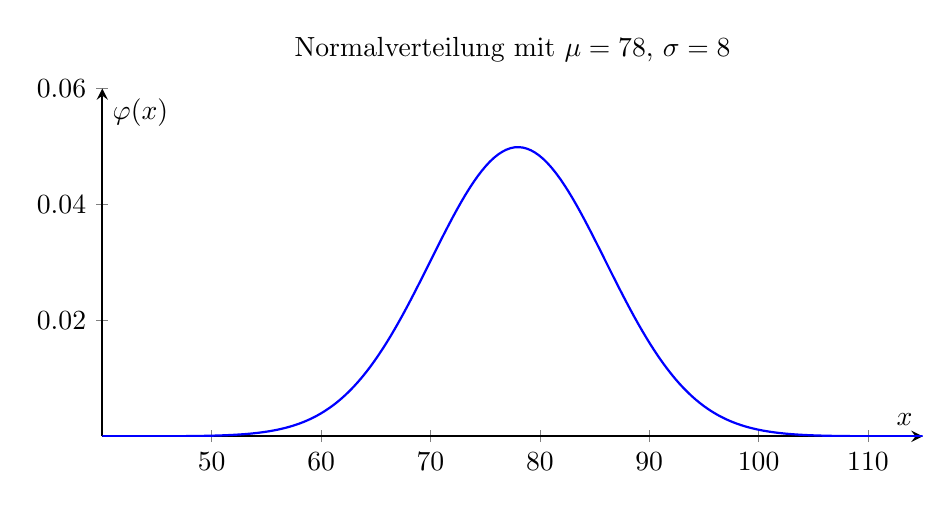
\begin{tikzpicture}
    \begin{axis}[
        width=12cm,
        height=6cm,
        domain=40:115,
        samples=200,
        xlabel={$x$},
        ylabel={$\varphi(x)$},
        xmin=40, xmax=115,      
        ymin=0, ymax=0.06, 
        title={Normalverteilung mit $\mu=78$, $\sigma=8$},
        thick,
        axis lines=middle,
        y tick label style={
            /pgf/number format/fixed,
            /pgf/number format/precision=4
        },
        x tick label style={
            /pgf/number format/use comma,
            /pgf/number format/precision=0
        },
        scaled ticks=false % verhindert 1e−4 Darstellung
    ]
        \addplot[blue] {1/(8*sqrt(2*pi)) * exp(-((x-78)^2)/(2*8^2))};
    \end{axis}
\end{tikzpicture}

\end{document}